\documentclass{beamer}
%\usepackage{beamerarticle}
\usepackage{tikz}
\usetikzlibrary{arrows,shapes}

\author{S.Poss and A.Sailer}
\title{Luminosity Spectrum Measurement}
\subtitle{Update}

\mode<presentation>
{
   \setbeamertemplate{navigation symbols}{}
   \setbeamertemplate{footline}[frame number] 
}

\AtBeginSection[]
{
\begin{frame}<beamer>
\frametitle{Outline}
\tableofcontents[currentsection,currentsubsection]
\end{frame}
}


\begin{document}
\begin{frame}
\titlepage 
\end{frame}
\begin{frame}
\frametitle{Outline}
\tableofcontents
% You might wish to add the option [pausesections]
\end{frame}

\begin{frame}
\frametitle{Introduction}
Last time:
\begin{itemize}
  \item Luminosity spectrum was not looking very good
  \item Some bugs found just before the meeting
\end{itemize}
Today:
\begin{itemize}
  \item Issues sorted out
  \item ``Final'' results for the CDR
  \item Some exercises with energy smearing 
\end{itemize}
\end{frame}

\section{Issues}
\begin{frame}
\frametitle{Issues found}
\begin{itemize}
  \item GuineaPig files were sorted, now use the unsorted ones
  \item One normalization parameter unnecessary removed
  \item For the 2D spectrum: not enough statistics when producing the files
  $\to$ unphysical file contents (Philipp)
\end{itemize}
\end{frame}

\section{CDR results}
\begin{frame}
\frametitle{CDR results: no energy smearing}
\centering
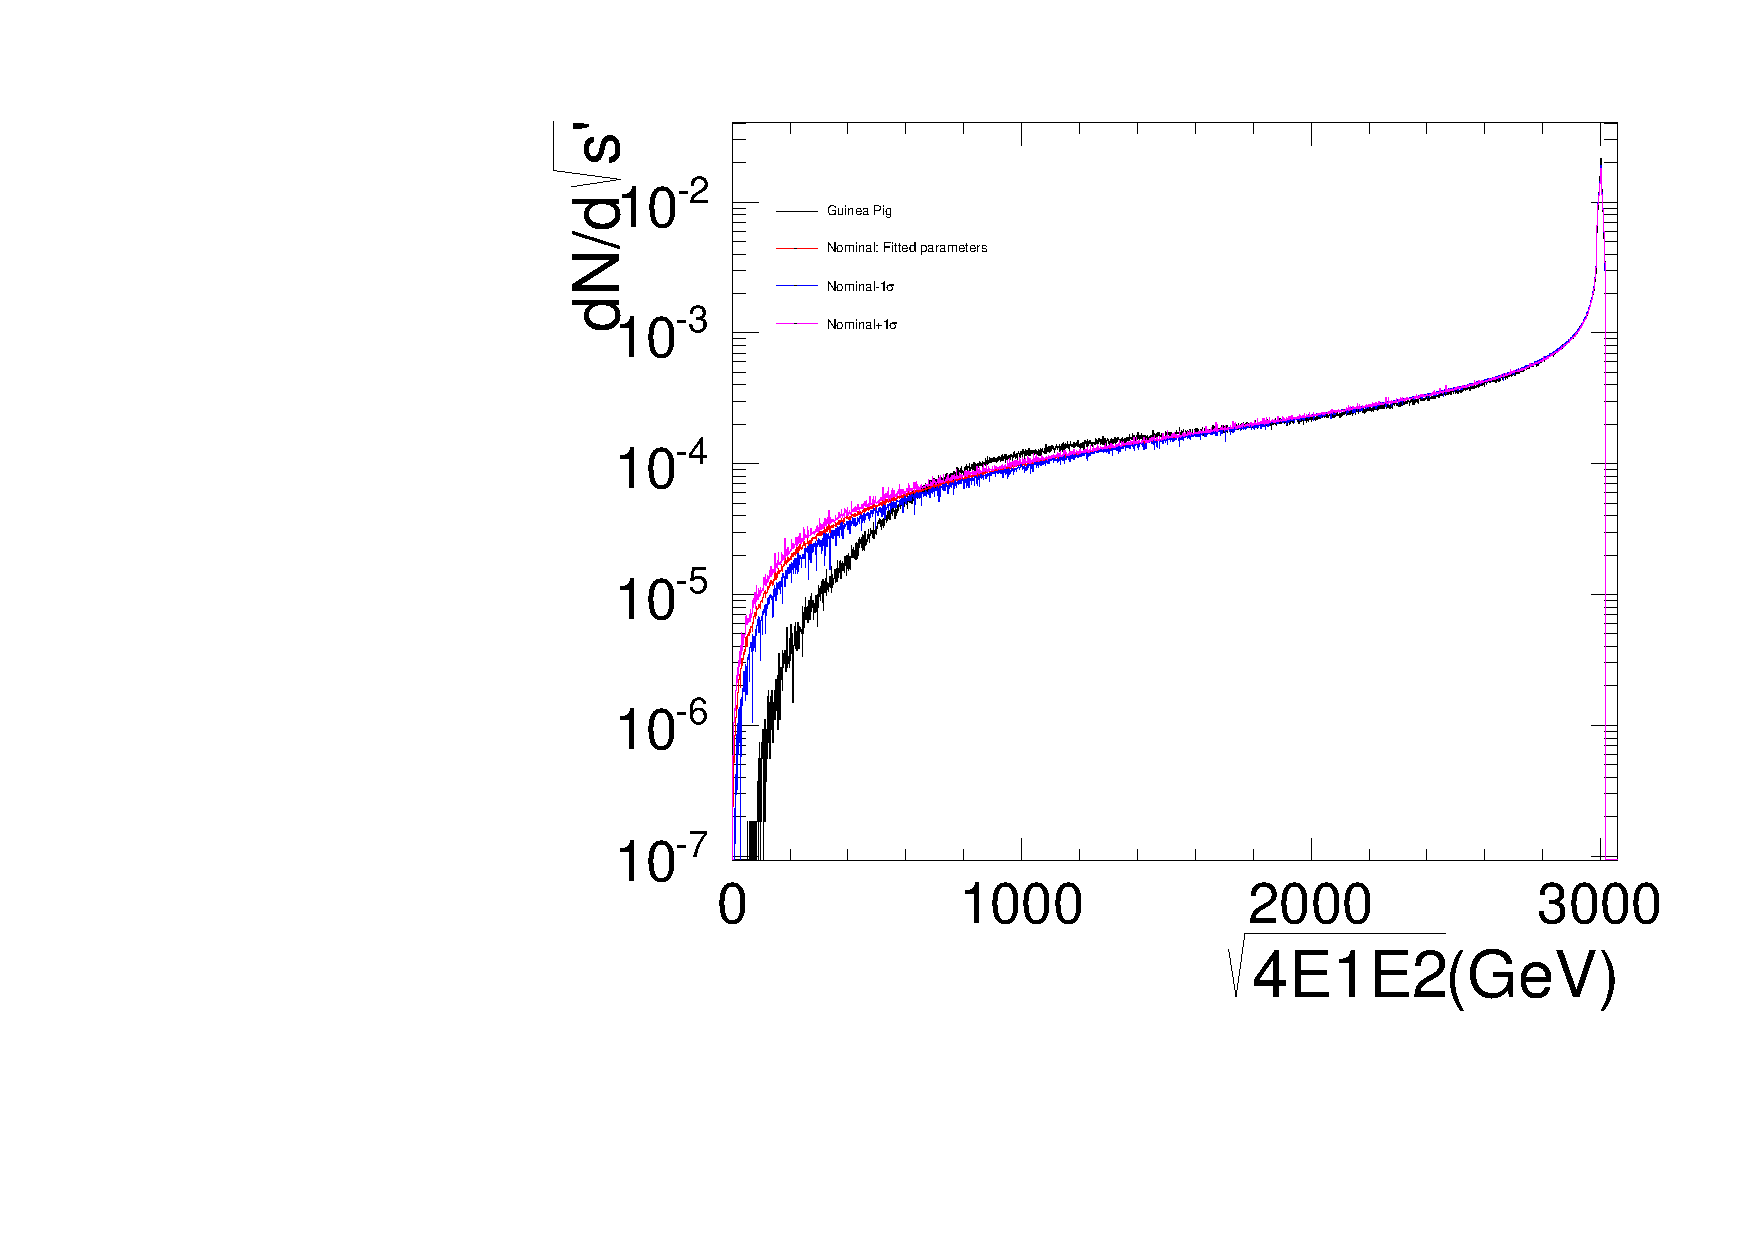
\includegraphics[width=9cm,page=1]{Spectra_BHWide_noEsmearing}
\end{frame}
\begin{frame}
\frametitle{CDR results: no energy smearing}
\centering
\includegraphics[width=9cm,page=2]{Spectra_BHWide_noEsmearing}
\end{frame}
\begin{frame}
\frametitle{CDR results: no energy smearing}
\centering
\includegraphics[width=9cm,page=4]{Spectra_BHWide_noEsmearing}
\end{frame}
\begin{frame}
\frametitle{CDR results: no energy smearing}
\centering
\includegraphics[width=9cm,page=3]{Spectra_BHWide_noEsmearing}
\end{frame}

\section{Playing with energy smearing}
\begin{frame}
\frametitle{Playing with energy smearing: $\frac{\sigma(E)}{E}=15\%/\sqrt{E}$}
\centering
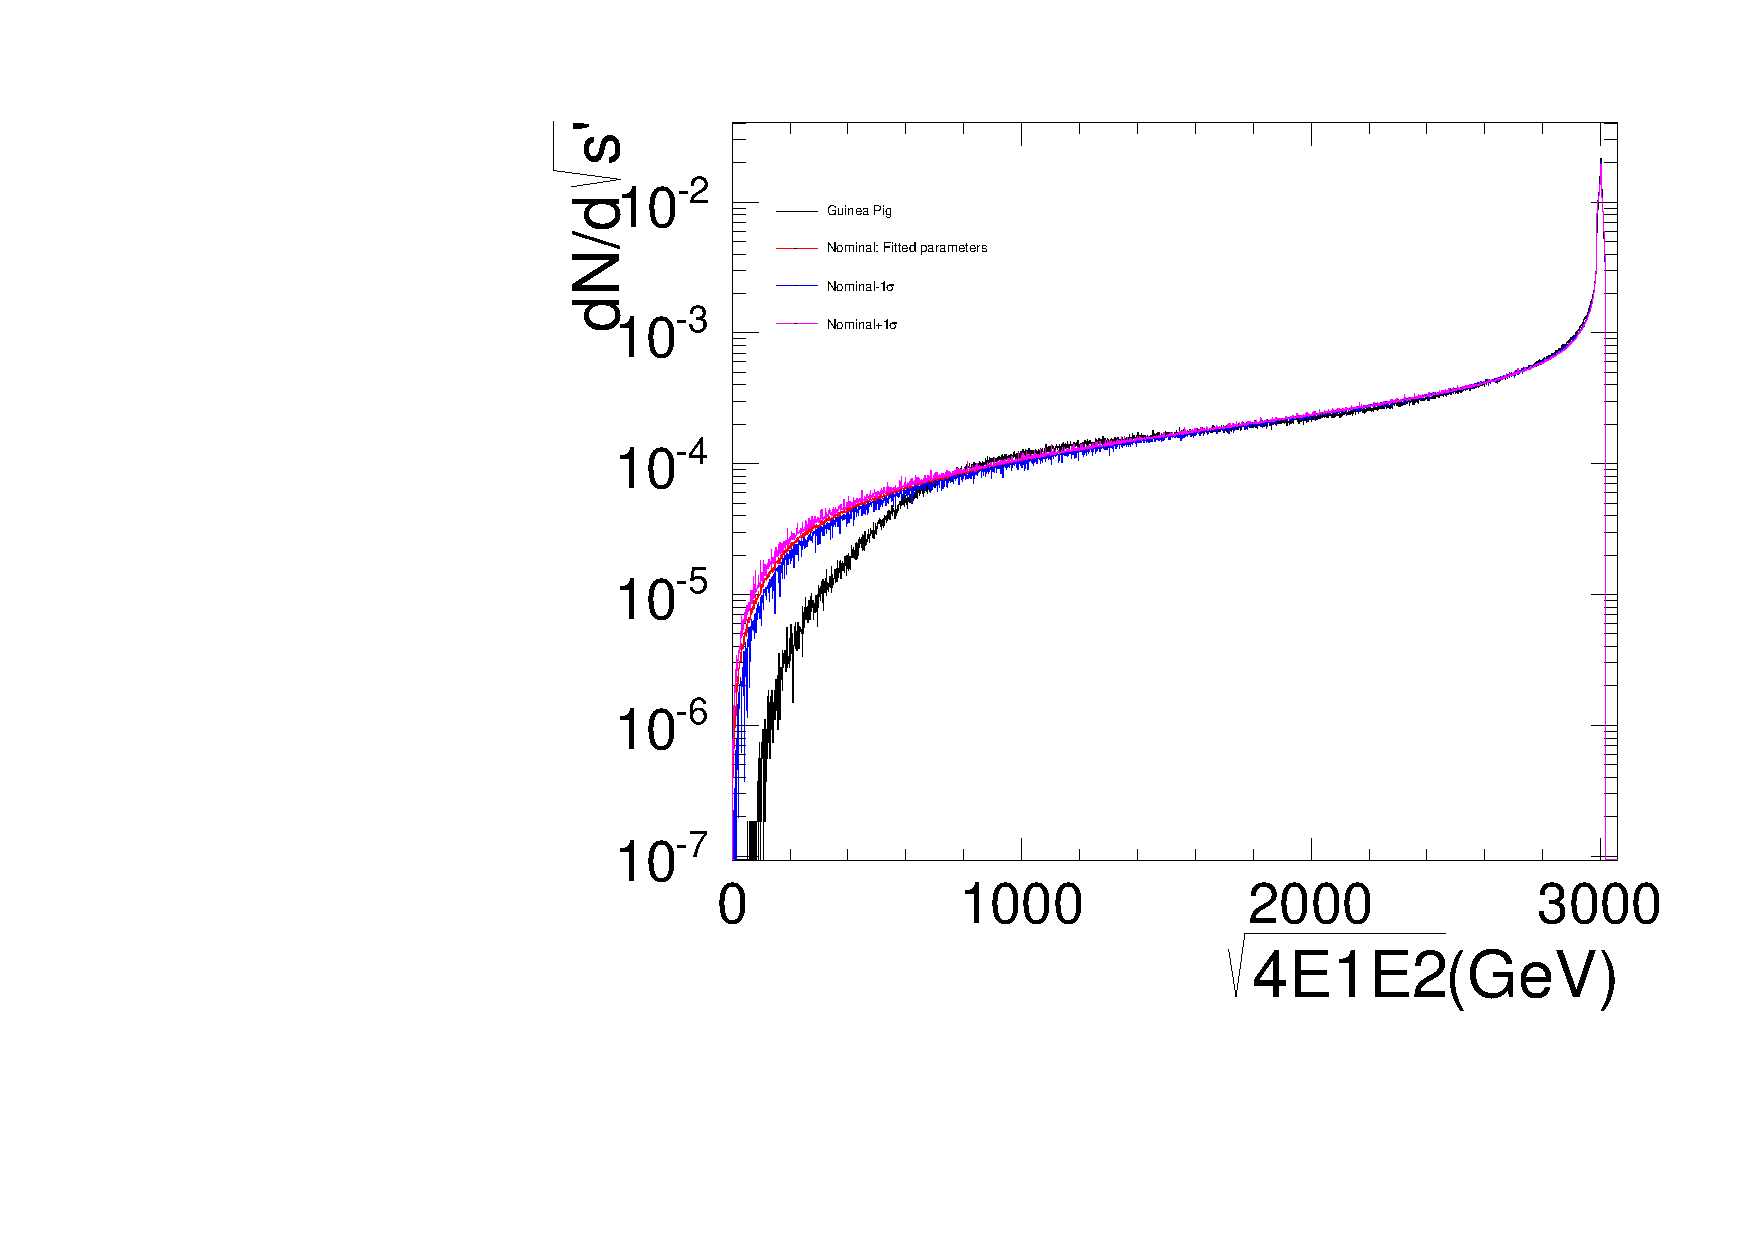
\includegraphics[width=9cm,page=1]{./Spectra_BHWide_Esmeared15.pdf}
\end{frame}
\begin{frame}
\frametitle{Playing with energy smearing: $\frac{\sigma(E)}{E}=15\%/\sqrt{E}$}
\centering
\includegraphics[width=9cm,page=2]{./Spectra_BHWide_Esmeared15.pdf}
\end{frame}
\begin{frame}
\frametitle{Playing with energy smearing: $\frac{\sigma(E)}{E}=15\%/\sqrt{E}$}
\centering
\includegraphics[width=9cm,page=4]{./Spectra_BHWide_Esmeared15.pdf}
\end{frame}
\begin{frame}
\frametitle{Playing with energy smearing: $\frac{\sigma(E)}{E}=15\%/\sqrt{E}$}
\centering
\includegraphics[width=9cm,page=3]{./Spectra_BHWide_Esmeared15.pdf}
\end{frame}
\begin{frame}
\frametitle{Playing with energy smearing: $\frac{\sigma(E)}{E}=15\%/\sqrt{E}$}
\begin{itemize}
  \item Energy smearing does not affect the tails
  \item ``Bump'' in peak introduced: 30\% deviation for 5GeV
\end{itemize} 
\end{frame}
\begin{frame}
\frametitle{Playing with energy smearing:
$\frac{\sigma(E)}{E}=20\%/\sqrt{E}\oplus0.5\%$}
\centering
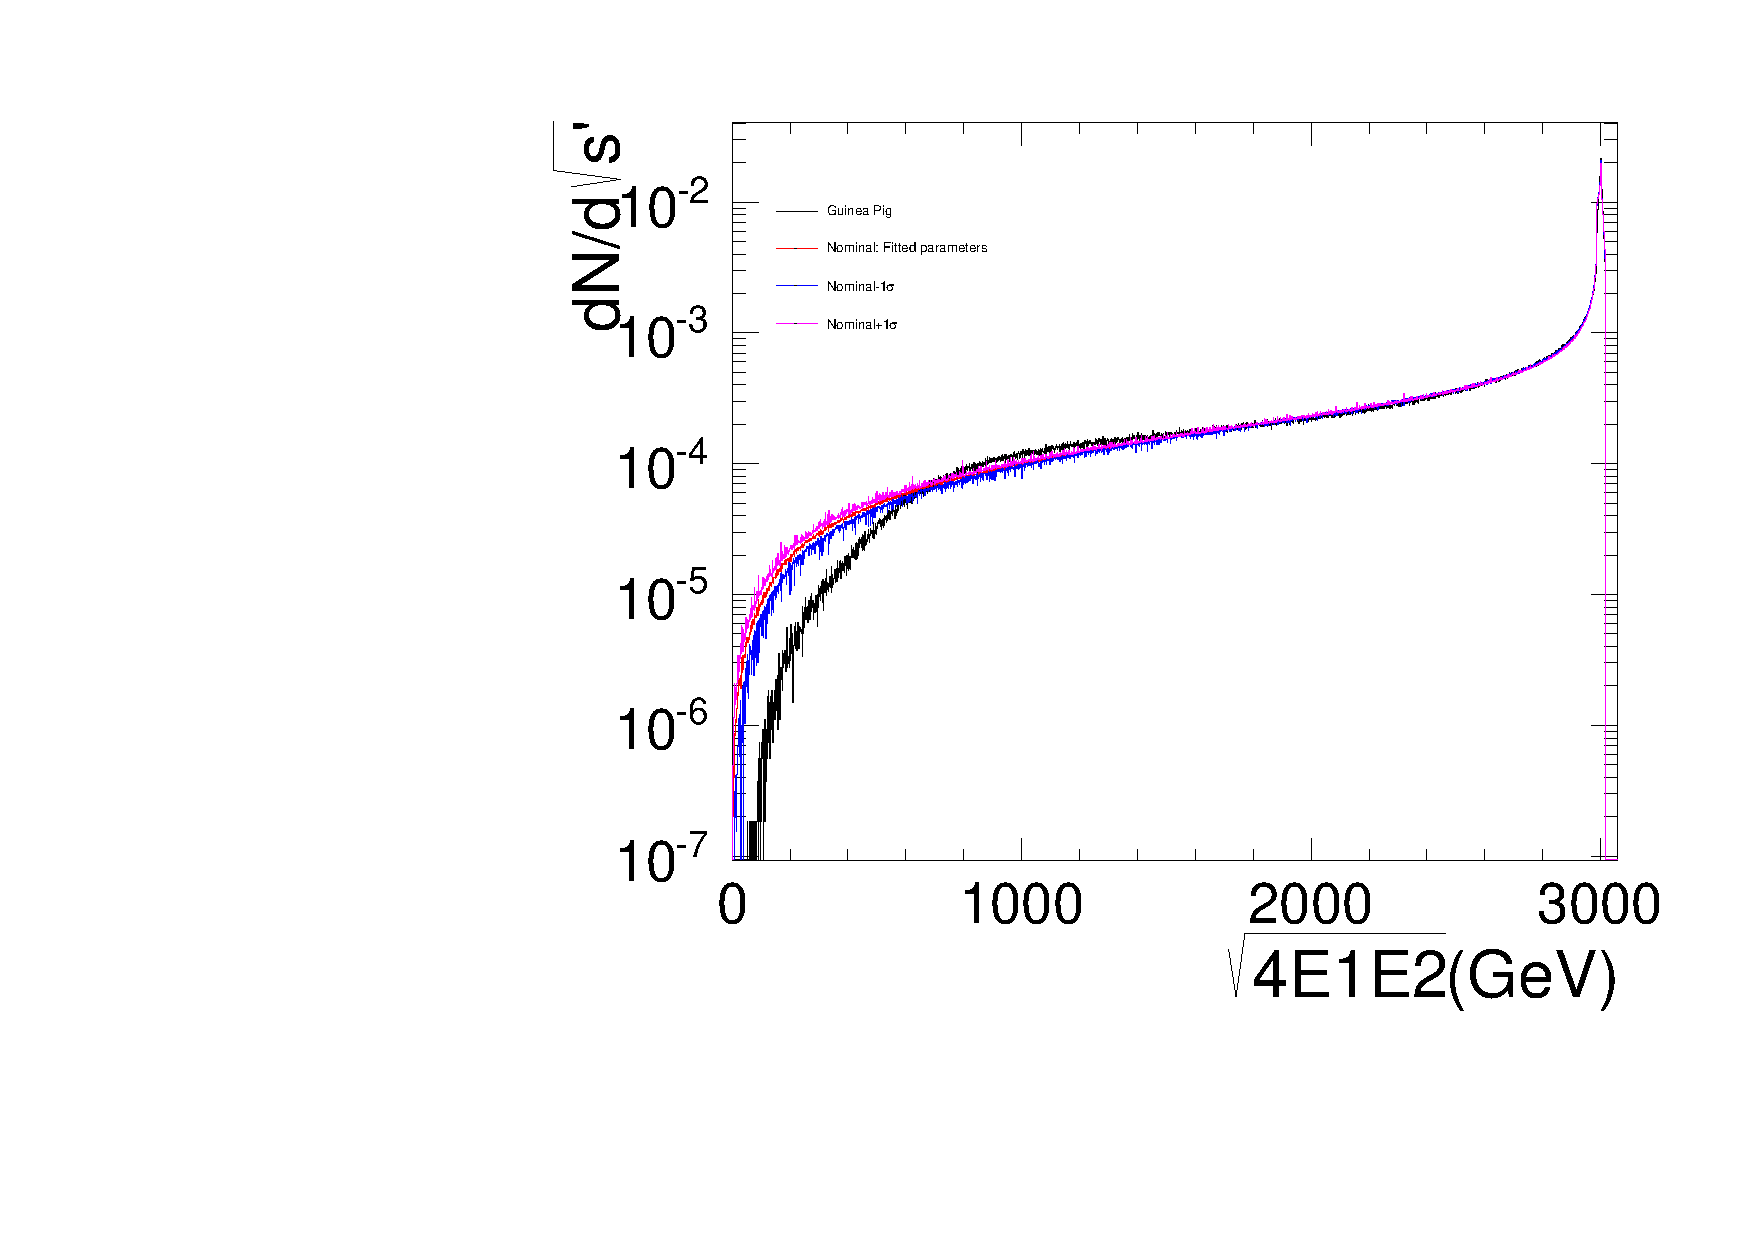
\includegraphics[width=9cm,page=1]{Spectra_BHWide_Esmeared20005.pdf}
\end{frame}
\begin{frame}
\frametitle{Playing with energy smearing:
$\frac{\sigma(E)}{E}=20\%/\sqrt{E}\oplus0.5\%$}
\centering
\includegraphics[width=9cm,page=2]{Spectra_BHWide_Esmeared20005.pdf}
\end{frame}
\begin{frame}
\frametitle{Playing with energy smearing:
$\frac{\sigma(E)}{E}=20\%/\sqrt{E}\oplus0.5\%$}
\centering
\includegraphics[width=9cm,page=4]{Spectra_BHWide_Esmeared20005.pdf}
\end{frame}
\begin{frame}
\frametitle{Playing with energy smearing:
$\frac{\sigma(E)}{E}=20\%/\sqrt{E}\oplus0.5\%$}
\centering
\includegraphics[width=9cm,page=3]{Spectra_BHWide_Esmeared20005.pdf}
\end{frame}
\begin{frame}
\frametitle{Playing with energy smearing:
$\frac{\sigma(E)}{E}=20\%/\sqrt{E}\oplus0.5\%$}
\begin{itemize}
  \item Bigger energy smearing does not affect the tails more than previous
  \item ``Bump'' in peak enhanced: 44\% deviation for 5GeV, other bins 
  $\sim10\%$ deviation
\end{itemize}
This requires additional modifications in model. 
\end{frame}

\section{Simplifying the model}
\begin{frame}
\frametitle{Simplify the model: assume symmetrical beams}
Why?
\begin{itemize}
  \item Because both beams are produced using the same simulation software
  \item Because many parameters and few events don't go well together: Not
  visible on 1D plots, but fitted beams are asymmetrical. For Philipp, this is
  essential
\end{itemize}
Realistic?
\begin{itemize}
  \item No! In ``real life'' the 2 beams will be sensibly different
  \item Statistics will not be a problem 
\end{itemize}
~\\
Exercise done with energy smearing: $\sigma(E)/E = 15\%/\sqrt{E}$.
\end{frame}
\begin{frame}
\frametitle{Simplify the model: assume symmetrical beams}
\includegraphics[width=9cm,page=1]{Spectra_all_BHWide_BHWideTuples_3e5sym.pdf}
\end{frame}
\begin{frame}
\frametitle{Simplify the model: assume symmetrical beams}
\includegraphics[width=9cm,page=2]{Spectra_all_BHWide_BHWideTuples_3e5sym.pdf}
\end{frame}
\begin{frame}
\frametitle{Simplify the model: assume symmetrical beams}
\includegraphics[width=9cm,page=4]{Spectra_all_BHWide_BHWideTuples_3e5sym.pdf}
\end{frame}
\begin{frame}
\frametitle{Simplify the model: assume symmetrical beams}
\includegraphics[width=9cm,page=3]{Spectra_all_BHWide_BHWideTuples_3e5sym.pdf}
\end{frame}

\section{Conclusion}
\begin{frame}
\frametitle{Conclusion}
\begin{itemize}
  \item Most problems fixed
  \item The energy smearing introduces a ``bump'': does it affect the
  measurements?
  \item Chosen not to show those spectra in the CDR, only those without energy
  smearing
  \item More analysis needed: full sim/reco for realistic energy measurement,
  systematics
  \item Will prepare note next year
\end{itemize}
\end{frame}
\end{document}